
%% bare_conf_compsoc.tex
%% V1.4b
%% 2015/08/26
%% by Michael Shell  
%% See:
%% http://www.michaelshell.org/
%% for current contact information.
%%
%% This is a skeleton file demonstrating the use of IEEEtran.cls
%% (requires IEEEtran.cls version 1.8b or later) with an IEEE Computer
%% Society conference paper.
%%
%% Support sites:
%% http://www.michaelshell.org/tex/ieeetran/
%% http://www.ctan.org/pkg/ieeetran
%% and
%% http://www.ieee.org/ 

%%*************************************************************************
%% Legal Notice:
%% This code is offered as-is without any warranty either expressed or
%% implied; without even the implied warranty of MERCHANTABILITY or
%% FITNESS FOR A PARTICULAR PURPOSE! 
%% User assumes all risk.
%% In no event shall the IEEE or any contributor to this code be liable for
%% any damages or losses, including, but not limited to, incidental,
%% consequential, or any other damages, resulting from the use or misuse
%% of any information contained here.
%%
%% All comments are the opinions of their respective authors and are not
%% necessarily endorsed by the IEEE.
%%
%% This work is distributed under the LaTeX Project Public License (LPPL)
%% ( http://www.latex-project.org/ ) version 1.3, and may be freely used,
%% distributed and modified. A copy of the LPPL, version 1.3, is included
%% in the base LaTeX documentation of all distributions of LaTeX released
%% 2003/12/01 or later.
%% Retain all contribution notices and credits.
%% ** Modified files should be clearly indicated as such, including  **
%% ** renaming them and changing author support contact information. **
%%*************************************************************************


% *** Authors should verify (and, if needed, correct) their LaTeX system  ***
% *** with the testflow diagnostic prior to trusting their LaTeX platform ***
% *** with production work. The IEEE's font choices and paper sizes can   ***
% *** trigger bugs that do not appear when using other class files.       ***                          ***
% The testflow support page is at:
% http://www.michaelshell.org/tex/testflow/



\documentclass[conference,compsoc]{IEEEtran}
% Some/most Computer Society conferences require the compsoc mode option,
% but others may want the standard conference format.
%
% If IEEEtran.cls has not been installed into the LaTeX system files,
% manually specify the path to it like:
% \documentclass[conference,compsoc]{../sty/IEEEtran}





% Some very useful LaTeX packages include:
% (uncomment the ones you want to load)


% *** MISC UTILITY PACKAGES ***
%
%\usepackage{ifpdf}
% Heiko Oberdiek's ifpdf.sty is very useful if you need conditional
% compilation based on whether the output is pdf or dvi.
% usage:
% \ifpdf
%   % pdf code
% \else
%   % dvi code
% \fi
% The latest version of ifpdf.sty can be obtained from:
% http://www.ctan.org/pkg/ifpdf
% Also, note that IEEEtran.cls V1.7 and later provides a builtin
% \ifCLASSINFOpdf conditional that works the same way.
% When switching from latex to pdflatex and vice-versa, the compiler may
% have to be run twice to clear warning/error messages.






% *** CITATION PACKAGES ***
%
\ifCLASSOPTIONcompsoc
  % IEEE Computer Society needs nocompress option
  % requires cite.sty v4.0 or later (November 2003)
  \usepackage[nocompress]{cite}
\else
  % normal IEEE
  \usepackage{cite}
\fi
% cite.sty was written by Donald Arseneau
% V1.6 and later of IEEEtran pre-defines the format of the cite.sty package
% \cite{} output to follow that of the IEEE. Loading the cite package will
% result in citation numbers being automatically sorted and properly
% "compressed/ranged". e.g., [1], [9], [2], [7], [5], [6] without using
% cite.sty will become [1], [2], [5]--[7], [9] using cite.sty. cite.sty's
% \cite will automatically add leading space, if needed. Use cite.sty's
% noadjust option (cite.sty V3.8 and later) if you want to turn this off
% such as if a citation ever needs to be enclosed in parenthesis.
% cite.sty is already installed on most LaTeX systems. Be sure and use
% version 5.0 (2009-03-20) and later if using hyperref.sty.
% The latest version can be obtained at:
% http://www.ctan.org/pkg/cite
% The documentation is contained in the cite.sty file itself.
%
% Note that some packages require special options to format as the Computer
% Society requires. In particular, Computer Society  papers do not use
% compressed citation ranges as is done in typical IEEE papers
% (e.g., [1]-[4]). Instead, they list every citation separately in order
% (e.g., [1], [2], [3], [4]). To get the latter we need to load the cite
% package with the nocompress option which is supported by cite.sty v4.0
% and later.





% *** GRAPHICS RELATED PACKAGES ***
%
\ifCLASSINFOpdf
  % \usepackage[pdftex]{graphicx}
  % declare the path(s) where your graphic files are
  % \graphicspath{{../pdf/}{../jpeg/}}
  % and their extensions so you won't have to specify these with
  % every instance of \includegraphics
  % \DeclareGraphicsExtensions{.pdf,.jpeg,.png}
\else
  % or other class option (dvipsone, dvipdf, if not using dvips). graphicx
  % will default to the driver specified in the system graphics.cfg if no
  % driver is specified.
  % \usepackage[dvips]{graphicx}
  % declare the path(s) where your graphic files are
  % \graphicspath{{../eps/}}
  % and their extensions so you won't have to specify these with
  % every instance of \includegraphics
  % \DeclareGraphicsExtensions{.eps}
\fi
% graphicx was written by David Carlisle and Sebastian Rahtz. It is
% required if you want graphics, photos, etc. graphicx.sty is already
% installed on most LaTeX systems. The latest version and documentation
% can be obtained at: 
% http://www.ctan.org/pkg/graphicx
% Another good source of documentation is "Using Imported Graphics in
% LaTeX2e" by Keith Reckdahl which can be found at:
% http://www.ctan.org/pkg/epslatex
%
% latex, and pdflatex in dvi mode, support graphics in encapsulated
% postscript (.eps) format. pdflatex in pdf mode supports graphics
% in .pdf, .jpeg, .png and .mps (metapost) formats. Users should ensure
% that all non-photo figures use a vector format (.eps, .pdf, .mps) and
% not a bitmapped formats (.jpeg, .png). The IEEE frowns on bitmapped formats
% which can result in "jaggedy"/blurry rendering of lines and letters as
% well as large increases in file sizes.
%
% You can find documentation about the pdfTeX application at:
% http://www.tug.org/applications/pdftex


\usepackage{pgfplots}
\usepackage{amssymb}
\usepackage{url}
\usepackage{enumitem}
\usepackage[linesnumbered,ruled]{algorithm2e}
\usepackage[export]{adjustbox}
\usepackage{xspace}
\usepackage{breqn}

\newtheorem{example}{Example}
\newtheorem{problem}{Problem}
\newtheorem{definition}{Definition}

\newcommand{\framework}{{\sc GeoGuide}}
\newcommand{\pb}{{\sc GeoGuide}}


% correct bad hyphenation here
\hyphenation{op-tical net-works semi-conduc-tor}


\begin{document}
%
% paper title
% Titles are generally capitalized except for words such as a, an, and, as,
% at, but, by, for, in, nor, of, on, or, the, to and up, which are usually
% not capitalized unless they are the first or last word of the title.
% Linebreaks \\ can be used within to get better formatting as desired.
% Do not put math or special symbols in the title.
\title{GeoGuide: An Interactive Guidance Approach for Spatial	Data}


\author{
    \IEEEauthorblockN{Pl\'acido A. Souza Neto\IEEEauthorrefmark{1}, Behrooz Omidvar-Tehrani\IEEEauthorrefmark{2}, Felipe M. Freire Pontes\IEEEauthorrefmark{3}, Francisco Bento\IEEEauthorrefmark{3}}
    \IEEEauthorblockA{\IEEEauthorrefmark{1}\IEEEauthorrefmark{3}Federal Institute of Rio Grande do Norte - IFRN, Brazil
    \\\IEEEauthorrefmark{1}placido.neto@ifrn.edu.br, \IEEEauthorrefmark{3}\{freire.pontes, bento.francisco\}@academico.ifrn.edu.br}
    \IEEEauthorblockA{\IEEEauthorrefmark{2}The Ohio State University, USA
    \\\IEEEauthorrefmark{2}omidvar-tehrani.1@osu.edu}
}

% conference papers do not typically use \thanks and this command
% is locked out in conference mode. If really needed, such as for
% the acknowledgment of grants, issue a \IEEEoverridecommandlockouts
% after \documentclass

% for over three affiliations, or if they all won't fit within the width
% of the page (and note that there is less available width in this regard for
% compsoc conferences compared to traditional conferences), use this
% alternative format:
% 
%\author{\IEEEauthorblockN{Michael Shell\IEEEauthorrefmark{1},
%Homer Simpson\IEEEauthorrefmark{2},
%James Kirk\IEEEauthorrefmark{3}, 
%Montgomery Scott\IEEEauthorrefmark{3} and
%Eldon Tyrell\IEEEauthorrefmark{4}}
%\IEEEauthorblockA{\IEEEauthorrefmark{1}School of Electrical and Computer Engineering\\
%Georgia Institute of Technology,
%Atlanta, Georgia 30332--0250\\ Email: see http://www.michaelshell.org/contact.html}
%\IEEEauthorblockA{\IEEEauthorrefmark{2}Twentieth Century Fox, Springfield, USA\\
%Email: homer@thesimpsons.com}
%\IEEEauthorblockA{\IEEEauthorrefmark{3}Starfleet Academy, San Francisco, California 96678-2391\\
%Telephone: (800) 555--1212, Fax: (888) 555--1212}
%\IEEEauthorblockA{\IEEEauthorrefmark{4}Tyrell Inc., 123 Replicant Street, Los Angeles, California 90210--4321}}




% use for special paper notices
%\IEEEspecialpapernotice{(Invited Paper)}




% make the title area
\maketitle

% As a general rule, do not put math, special symbols or citations
% in the abstract
\begin{abstract}
Spatial data is becoming increasingly available in various domains such as transportation and social science. Discovering patterns and trends in this data provides improved insights for planning and decision making for smart city management, disaster management and other applications. However, exploratory analysis of such data is a challenge due to its huge size of spatial data. It is often unclear for the analyst {\em what to see next} during an analysis process, i.e., lack of guidance. To tackle this challenge, we develop \framework, an interactive guidance approach for spatial data. \framework\ captures the implicit feedback of analyst and exploits it to highlight potentially interesting analysis options. Demo attendees will experience \framework\ in various datasets from restaurant check-ins to transportation.
\end{abstract}

% no keywords




% For peer review papers, you can put extra information on the cover
% page as needed:
% \ifCLASSOPTIONpeerreview
% \begin{center} \bfseries EDICS Category: 3-BBND \end{center}
% \fi
%
% For peerreview papers, this IEEEtran command inserts a page break and
% creates the second title. It will be ignored for other modes.
\IEEEpeerreviewmaketitle



\section{Introduction} 
Nowadays, there exists huge amounts of spatial data in various fields of science, such as agriculture, transportation and social science. Analysis of such data is interesting as it is grounded
on reality: each record represents a specific geographical location. Moreover, understanding patterns and trends provides insights leading to improved user planning and decision making. Some instance applications of spatial data are smart city management, disaster management and autonomous transport \cite{RoddickEHPS04,Telang:2012}.


Spatial data analysis is often performed in {\em exploratory context}: the analyst does not have a precise query in mind and she explores data in iterative steps in order to find potentially interesting results. Traditionally, an exploratory analysis scenario on spatial data is described as follows: the analyst visualizes a subset of data using a query in an off-the-shelf product (e.g., Tableau\footnote{\it http://www.tableau.com},
 Exhibit\footnote{\it http://www.simile-widgets.org/exhibit/},
Spotfire\footnote{\it http://spotfire.tibco.com}). The result will be illustrated on a geographical map. Then she investigates on different parts of the visualization by zooming in/out and panning the map in order to discover patterns and trends of interest. The analyst may iterate on this process several times by issuing different queries and focusing on different aspects of data. 



To overcome the challenge of value in exploratory analysis, visualization environments offer a complete tool-set to manipulate data (filter, aggregate, etc.). In practice, this duplicates the problem: the analyst is left alone in a huge space of spatial data and tools. The principled challenge for the analyst is {\em ``what to see next''} in the exploratory context. A {\em guidance} mechanism is then necessary to point out potential future directions of analysis.


 

The following example illustrates the challenge in practice.

\begin{example}
\label{ex:airbnb}
Liam is planning a short trip to Paris. He decides to rent a home-stay from Airbnb website\footnote{\it http://www.airbnb.com}. He is open to any type of lodging and he wants to explore different options (i.e., exploratory analysis). He queries all available locations in Paris with a fair price. His query results in 3000 locations. As he has no other preferences, an exhaustive investigation needs scanning each location independently which is nearly infeasible. In case he wants to focus on a smaller set of options, it is not clear which subset he needs to look at. While he is looking at primary locations in the list, he shows interest in having ``balcony'' as amenity and being close to Eiffel tower. An ideal system can capture this feedback in order to short-list a small subset of remaining locations that Liam should consider as high priority.
\end{example}

In order to contribute to overcome this challenge, we  propose \framework, an interactive framework to highlight a subset of geographical points based on analyst feedback. Although \framework\ operates on points, its functionality can be easily extended to regions using point-clustering methods. The highlighted set facilitates the decision-making process by providing guidance on what the analyst should potentially concentrate on. The set of highlights is deliberated over high quality. We consider two quality metrics in \framework: {\em relevance} and {\em diversity}. First, each highlighted point should be relevant to historical choices of the analyst. Second, highlights should be geographically diverse to unveil different aspects of analysis. Both quality metrics are interdependent to compute the set of highlights.

Despite literature contains several instances of feedback exploitation to guide the analyst in further analysis steps (e.g., \cite{boley2013one}), the common used approach is the top-$k$ processing methodology in order to prune the search space based on the explicit feedback and recommend a small subset of interesting results of size~$k$. A clear distinction and contribution of \framework\ is that it doesn't aim for pruning, but leveraging the actual data with potential interesting results that the analyst may miss due to the huge volume of spatial data. While in top-$k$ processing algorithms, analyst choices are limited to $k$, \framework\ has a freedom of choice where highlights get seamlessly updated with new analyst choices. 


The literature in spatial data analysis also has a focus on {\em efficiency} of exploratory iterations: {\em ``how can analysts navigate in spatial data fluidly?''} The common approach is to design pre-computed indexes which enable efficient retrieval of spatial data (e.g., \cite{lins2013nanocubes}). However, there has been fewer attention to the {\em value} of spatial data. Despite the huge progress on efficiency front, an analyst may easily get lost in the plethora of geographical points because $i.$ she doesn't know what to investigate next in an exploratory context and $ii.$ she may get distracted and miss interesting points by visual clutter caused by huge point overlaps. In other words, although iteration transitions (between one analysis step to the other) can be performed efficiently, the decision which forms a transition, remains unclear.

There exist still few instances of information-highlighting methods in the literature \cite{Liang2010,Robinson2011,wongsuphasawat2016voyager,willett2007scented}. All these methods are {\em objective} and do not apply to the context of spatial guidance where user feedback is involved.  In terms of recommendation, few approaches focus on spatial dimension \cite{Bao2015,Levandoski:2012} while the context and result diversification are missing.

To better demonstrate our approach, we summarize the following sections: in Section \ref{sec:pb}  we present \framework\, and its associated concepts. Section \ref{sec:scenario}  presents the possible scenarios to run \framework\ . Section  \ref{sec:experiments}  shows some initial experiments and Section \ref{sec:conclusions}  presents some conclusions and future directions. 


\section{\framework\ Approach: Highlighting Spatial Data}
\label{sec:pb}

Given a dataset with a set of spatio-temporal information points, our system is able to process and generates highlighted informations base on analyst preferences and behaviour. Our proposed framework is able to highlight different information based on specific data attributes, highlighting, for instance, each points by size or color intensity. Using \framework\ framework the analyst can also define a subset of points to be highlighted over the dataset by a simple filtering action. The functionalities of \framework\ are an inspiration from both recommendation \cite{Omidvar-Tehrani:2015} and visual highlighting \cite{Liang2010,Robinson2011} methodologies. \framework\ is a layer on top of a raw visualization to guide analysts in large-scale spatial data analysis. Figure \ref{fig:framework} illustrates the main components of \framework\ architecture.


\begin{figure}[t]
  \centering
  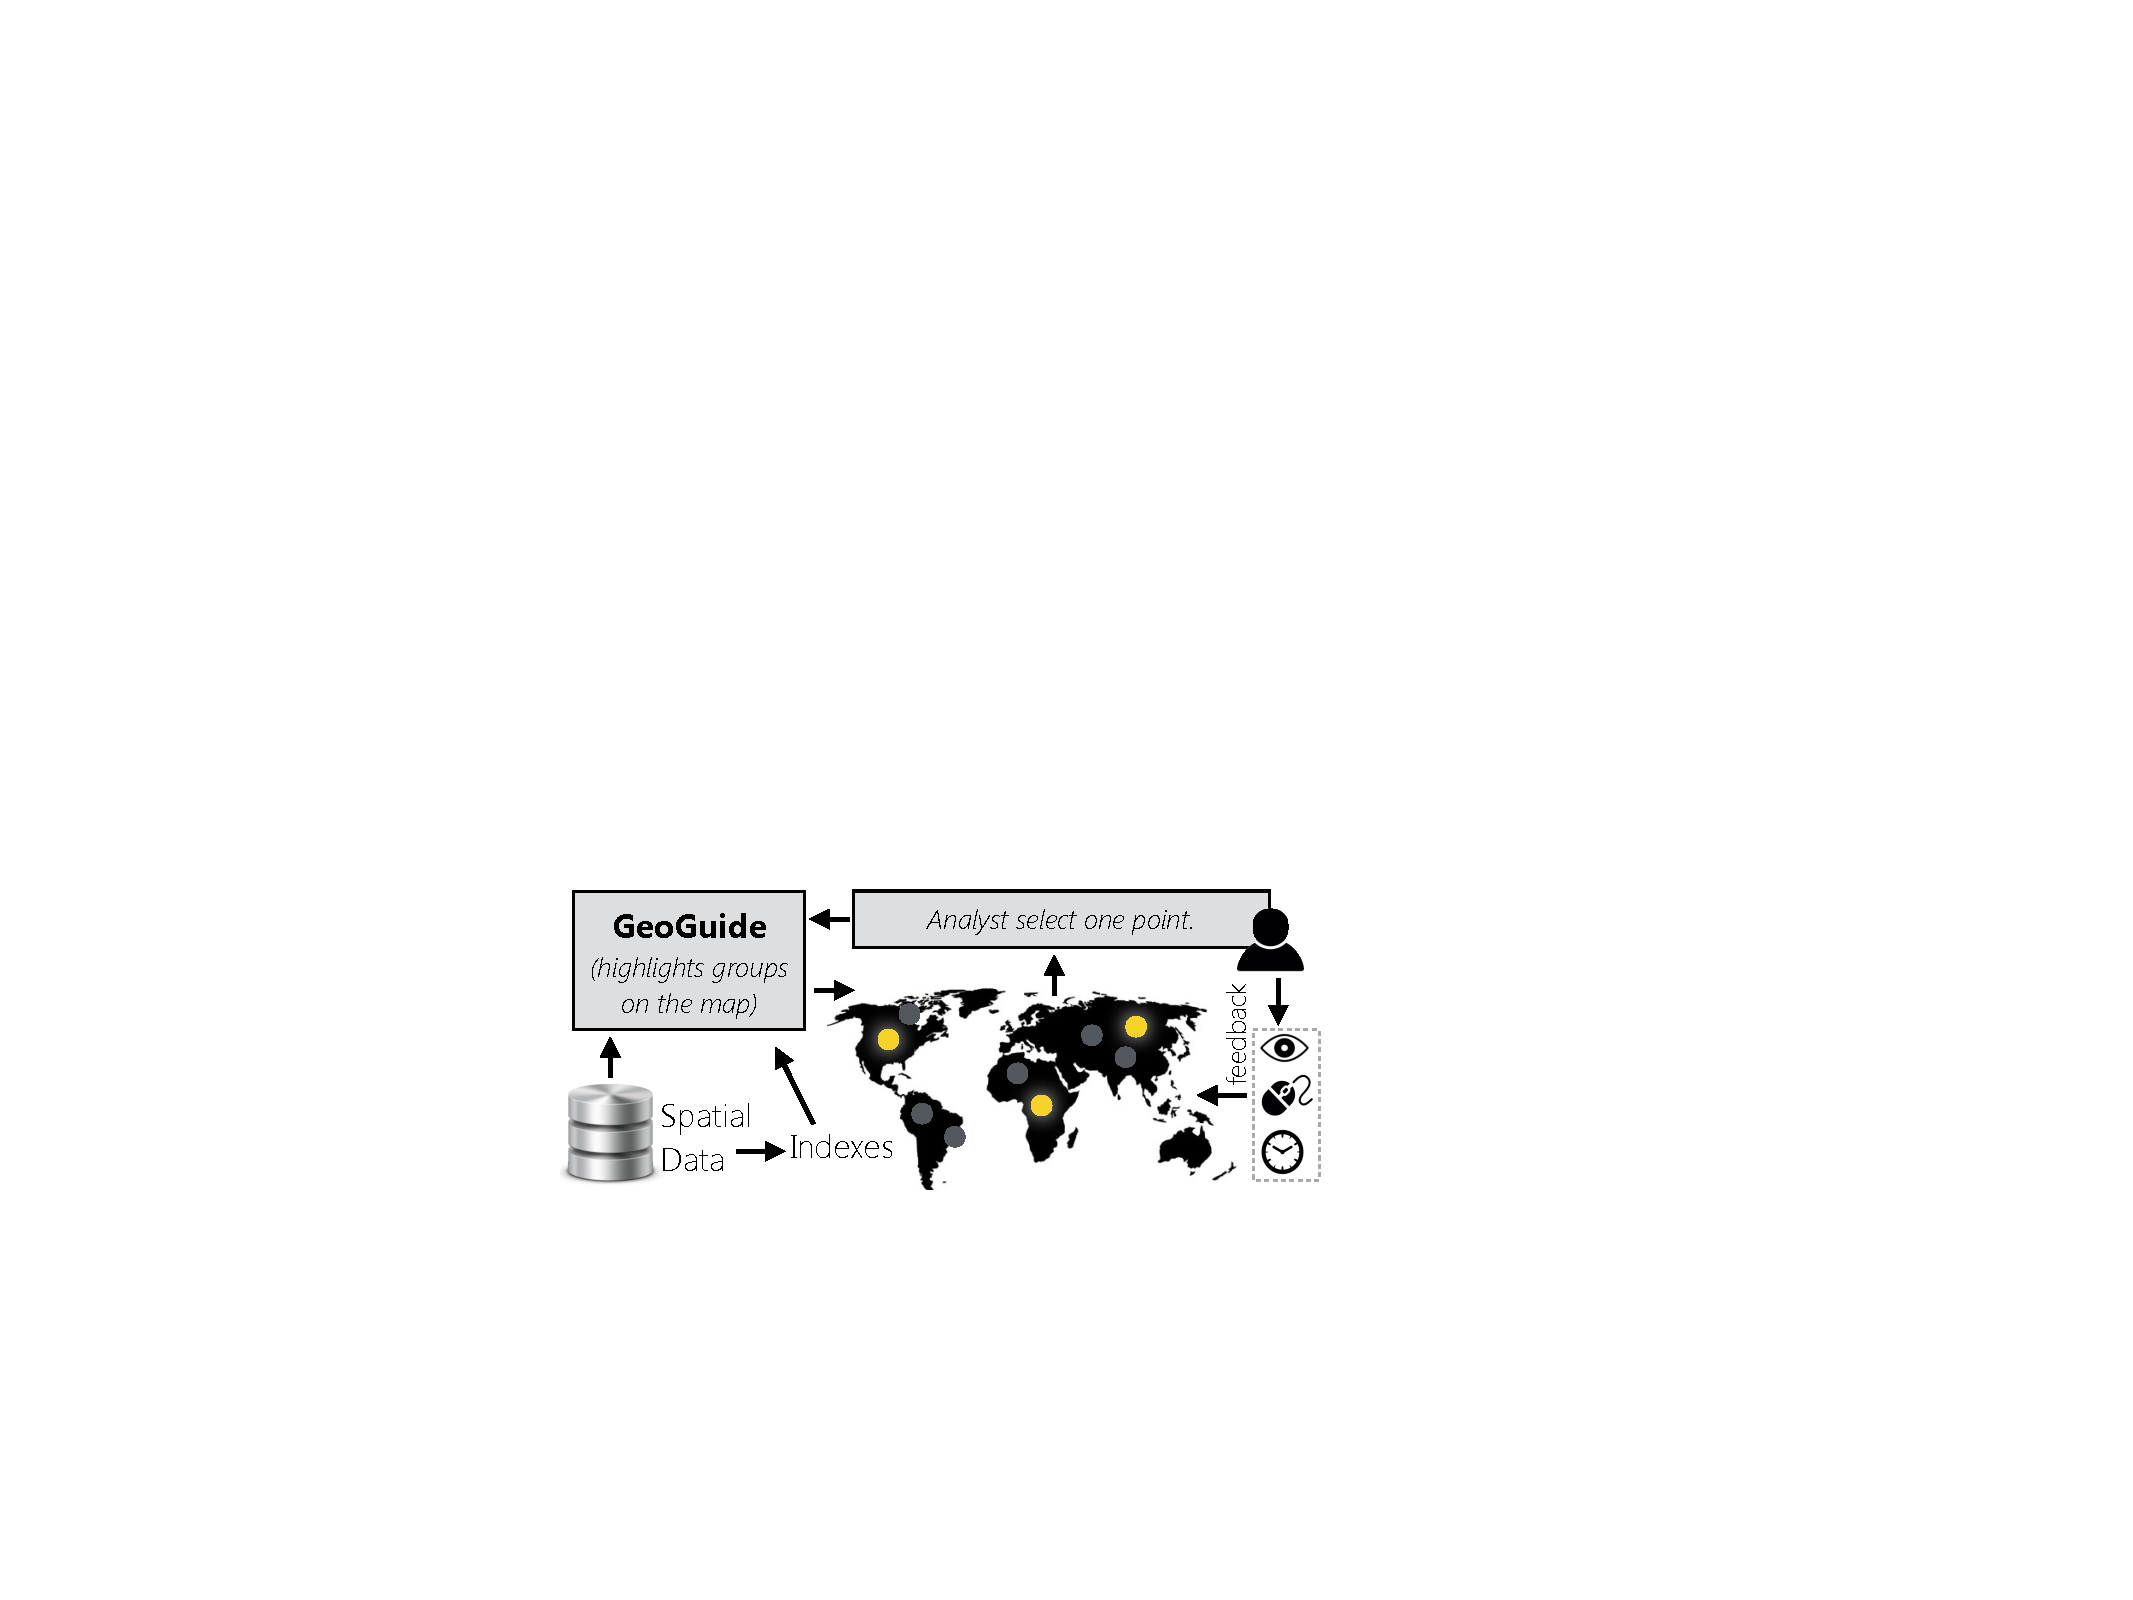
\includegraphics[width=\columnwidth]{figs/framework}
\caption{\framework\ Framework}
\label{fig:framework}
\vspace{-10pt}
\end{figure}

The following example describes an application of \framework\ in business domain.

\begin{example}
\label{ex:flight}
Tiffany is a data scientist and is tasked to design a ``chain marketing'' strategy for a Peking Duck product (a Chinese duck dish). She decides to exploit Yelp data\footnote{\it https://www.yelp.com/} (i.e., restaurant check-ins) to find out the advertisement chain. She performs her analysis in \framework. In the first step, she shows interest towards New York region, where the headquarters of the company is located and the product has already gained success. The system will then provide few highlights in diverse regions: San Fransisco, Washington DC and Marlton, NJ. All regions seem interesting to Tiffany as they exhibit similar eating profile with New York, hence potentials for chaining the advertisement. She decides to pick Marlton due to its proximity so that she can reduce transportation costs. The system will then provide other highlights based on her updated feedback. She can then make the city-to-city chain marketing strategy in iterative steps using highlights.
\end{example}


In our approach, we consider a spatial database ${\cal D}$ consisting $\langle {\cal P}, {\cal A} \rangle$ where ${\cal P}$ is the set of
geographical points and ${\cal A}$ is the set of point attributes. For each $p \in {\cal P}$, we consider a tuple $\langle lat, lon, alt\rangle$ which denotes $p$'s geographical coordinates (latitude, longitude and altitude respectively). The set ${\cal A}_p$ contains attribute-values for $p$ over the schema of ${\cal A}$. For instance, on a restaurant check-ins dataset, ${\cal A}_p = \langle${\tt female}, {\tt young}, {\tt chinese-food}$\rangle$ on the schema ${\cal A} = \langle${\tt gender}, {\tt age}, {\tt type}$\rangle$ denotes that $p$ is associated to a young female who likes chinese dish. The set ${\cal A}$ is domain-dependent and defines the semantics of a spatial dataset.


\subsection{Relevance and Diversity}

At each step of the analysis, \framework\ highlights few points based on the feedback content ${\cal F}$. The highlighting decision is made based on two quality metrics, i.e., relevance and diversity. 

\vspace{5pt}
\noindent {\bf Relevance.} Highlights should be in the same line with analyst feedback (captured either by gaze, mouse cursor or session time). Note that we consider {\em contextual-based} relevance and not {\em distance-based} relevance. The reason originates from our data observation. For instance in a taxi dataset, consider a ride in New York for a young male customer for an itinerary of 10 kilometers and \$3 tip. In contrary to thousands of kilometers of geographical distance, the ride is very relevant to another one in San Fransisco for a middle-age male customer for an itinerary of 8 kilometers and \$2.5 tip. The relevance between a point $p$ and the feedback vector ${\cal F}$ is defined as follows.

% \begin{definition}[Relevance]
% Given two points $p$ and $p'$ and their attribute values ${\cal A}_{p}$ and ${\cal A}_{p'}$, the relevance between $p$ and $p'$ is a value between $0$ and $1$ denoted as $\mathit{relevance}(p,p') = \mathit{average}_{a \in {\cal A}_{p} \cup {\cal A}_{p'}}(\mathit{sim({\cal A}_{p}, {\cal A}_{p'}, a)})$.
% \label{def:rel}
% \end{definition}

\begin{dmath}
	\label{eq:rel}
	\mathit{relevance}(p,{\cal F}) = \mathit{average}_{a \in {\cal A}_{p} \cap {\cal F}}(\mathit{sim(p, {\cal F}, a)})
\end{dmath}

The similarity function $\mathit{sim}()$ can be any function such as Jaccard and Cosine. Each attribute can have its own similarity function (as string and integer attributes are compared differently.) Then $\mathit{sim}()$ works as an overriding-function which provides encapsulated similarity computations for any type of attribute.

\vspace{5pt}
\noindent {\bf Diversity.} Highlighted points should also represent distinct regions so that the analyst can observe different aspects of data and decide based on the big picture. Given a set of points $s = \{ p_1, p_2 \dots \}$, we define {\em diversity} as follows.

\begin{dmath}
	\label{eq:divs}
	\mathit{diversity}(s) = \mathit{average}_{\{p, p'\} \subseteq s | p \neq p' } \mathit{distance}(p,p')
\end{dmath} 

The function $\mathit{distance}(p,p')$ operates on geographical coordinates of $p$ and $p'$ and can be considered as any distance function of Chebyshev distance family such as Eucledian. However, as distance computations are done in {\em spherical space} using latitude, longitude and altitude, it is au-naturel to employ Haversine distance shown in Equation \ref{eq:harvestine}.

\begin{dmath}
	\label{eq:harvestine}
	distance(p,p') = [ acos(cos(p_{lat}) . cos(p'_{lat}) . cos(p_{lon}) . cos(p'_{lon})\\ + cos(p_{lat}) . sin(p'_{lat}). cos(p_{lon}) . sin(p'_{lon}) + sin(p_{lat}) . sin(p'_{lat})) ] \times earth\_radius
\end{dmath}

% \vspace{5pt}
% Following aforementioned desiderata, we formulate highlighting as an optimization-based problem on relevance and diversity dimensions.

% \begin{problem}[\pb]
% \label{pb:geoh}
% Given an input point $p$ and a threshold $\sigma$, the problem is to return top-$k$
%  points denoted $S_p$ where $|S_p| = k$ and $\forall p' \in S_p, \mathit{relevance}(p,p') \geq \sigma$ and $\mathit{diversity}(S_p)$ is maximized.
% \end{problem}

% Problem \ref{pb:geoh} is hard due to the huge space of spatiotemporal data: for any given point $p$, an exhaustive search over all other points is necessary to find $k$ points with maximal relevance. Moreover, the problem investigates in two dimensions at the same time (relevance and diversity) which makes it more challenging.

\framework\ employs a best-effort greedy approach to efficiently compute highlighted points. We consider an offline step followed by the online execution of \framework.
In order to speed up computing relevance in online execution, we pre-compute an inverted index for each single geographical point in ${\cal P}$ in the offline step (as is commonly done in Web search). Each index ${\cal L}_p$ for the point $p$ keeps all other points in ${\cal P}$ in decreasing order of their relevance with $p$.

During online execution, \framework\ admits as input a point $p \in {\cal P}$ (the user explicit choice) and returns the set of highlights ${\cal H} \subset {\cal P}$. \framework\ makes sequential accesses to ${\cal L}_p$ to greedily maximize diversity. Points in ${\cal L}_p$ get a weight using ${\cal F}$. Points with a larger weight (i.e., closer to the analyst feedback) have a higher chance to be in ${\cal H}$. To speed up comparisons with ${\cal F}$ vector, we exploit bit-wise comparisons. We convert both ${\cal F}$ and point $p$ to boolean representations and compute relevance (Equation \ref{eq:rel}) using bit-wise operators.

\framework\ does not sacrifice efficiency in price of value. We consider a {\em time limit} parameter which determines when the algorithm should stop seeking maximized diversity. Scanning inverted indexes guarantees the relevance even if time limit is chosen to be very restrictive. Our observations with several datasets show that we achieve the diversity of more than $0.9$ with time limit set to $200ms$.

%\noindent{\bf Context.} 
\begin{figure*}[t]
	\centering
	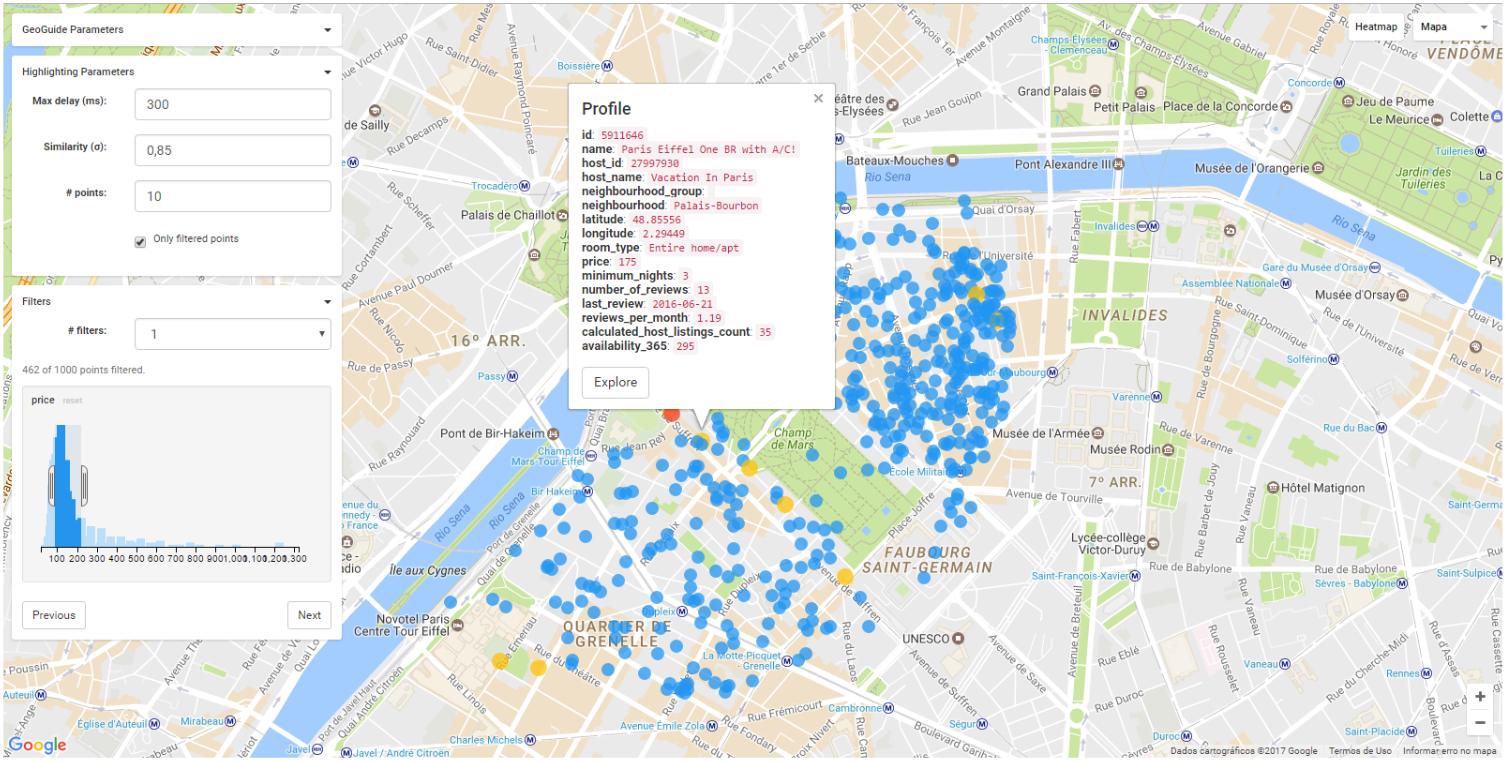
\includegraphics[width=\textwidth]{figs/airbnb}
	\caption{\framework\ Image on Airbnb Dataset - Paris City}
	\label{fig:airbnb}
	\vspace{-10pt}
\end{figure*}

\subsection{Algorithm}
\label{sec:algo}
We propose a solution for \pb\ by inspiring from both recommendation \cite{Omidvar-Tehrani:2015} and
visual highlighting
% \cite{Lohmann:2012,Robinson2011,Liang2010}
\cite{Liang2010,Robinson2011}
methodologies. \pb\ requires an efficient algorithm for dynamically analyzing and comparing geographical points. We propose \framework\ as a solution for the generic guidance problem in spatiotemporal data (Figure \ref{fig:framework}). Although \framework\ operates on points, its functionality can be easily extended to regions using point-clustering methods such as $k$-means.

\framework\ operates in two steps: {\sc Preparation} and {\sc Highlighter}. In order to speed up computing relevance in online execution, we pre-compute an inverted index for each single geographical point in ${\cal P}$ in the offline {\sc Preparation} step (as is commonly done in Web search). Each index ${\cal L}_p$ for the point $p$ stores all other points in ${\cal P}$ in decreasing order of their relevance with $p$. Thanks to the parameter $\sigma$, we only partially materialize the indexes.

% behrooz: explain the whole package

Algorithm \ref{algo:geoh} illustrates the online execution step of \framework\, so called {\sc Highlighter}. The algorithm is a single greedy procedure that solves the \pb\ problem. {\sc Highlighter} is called at each interactive step of \framework\ (as in Figure \ref{fig:framework}). The algorithm admits as input a point $p \in {\cal P}$ and returns the best $k$ points denoted ${\cal S}_p$.

%To comply with the desiderata {\bf D5}, we consider a time limit parameter $tlimit$ in Algorithm \ref{algo:geoh}. In a {\em best-effort} strategy, the algorithm bounds user waiting time by $tlimit$ to return the best possible results by then.

\begin{algorithm}[t]
	\DontPrintSemicolon
	\KwIn{$p \in {\cal P}$, $\sigma$, $k$, $tlimit$}
	% \KwOut{${\cal S}_p$}
	${\cal S}_p \gets get\_top\_k(\mathit{{\cal L}^p})$\;\label{cd:gettopk}
	$p_{next} \gets get\_next(\mathit{{\cal L}^p})$\;\label{cd:getnext}
	\While{$(tlimit$ $not$ $exceeded \wedge relevance(p,p_{next}) \geq \sigma)$}{\label{cd:beginwhile}
		\For{$p_{current} \in {\cal S}_p$}{
			\If{$\mathit{diversity\_improved}({\cal S}_p,p_{next},p_{current})$}{\label{cd:betterdiv}
				${\cal S}_p \gets \mathit{replace}({\cal S}_p,p_{next},p_{current})$\;
				$break$\;
			}
		}
		$p_{next} \gets get\_next({\cal L}^p)$\;}\label{cd:endwhile}
	\Return{${\cal S}_p$}\; 
	\caption{{\sc Highlighter} Algorithm}
	\label{algo:geoh}
\end{algorithm}
% \vspace{-10pt}
% behrooz: mention working of sacrification

{\sc Highlighter} begins by retrieving the most relevant points to $p$ by simply retrieving the $k$ highest ranking points in ${\cal L}_p$ (line \ref{cd:gettopk}). Function $get\_next({\cal L}_p)$ (Line \ref{cd:getnext}) returns the next point $p_{next}$ in ${\cal L}_p$ in sequential order. Lines \ref{cd:beginwhile} to \ref{cd:endwhile} iterate over the inverted indexes to determine if other points should be considered to increase diversity while staying within the time limit and not violating the relevance threshold with the selected point. Since points in ${\cal L}_g$ are sorted on decreasing relevance with $p$, the algorithm can safely stop as soon as the relevance condition is violated (or if the time limit is exceeded).

The algorithm then looks for a candidate point $p_{current} \in {\cal S}_p$ to replace in order to increase diversity. The boolean function $\mathit{diversity\_improved}()$ (line \ref{cd:betterdiv}) checks if by replacing $p_{current}$ by $p_{next}$ in ${\cal S}_p$, the overall diversity of the new ${\cal S}_p$ increases.


\begin{figure*}[t]
	\centering
	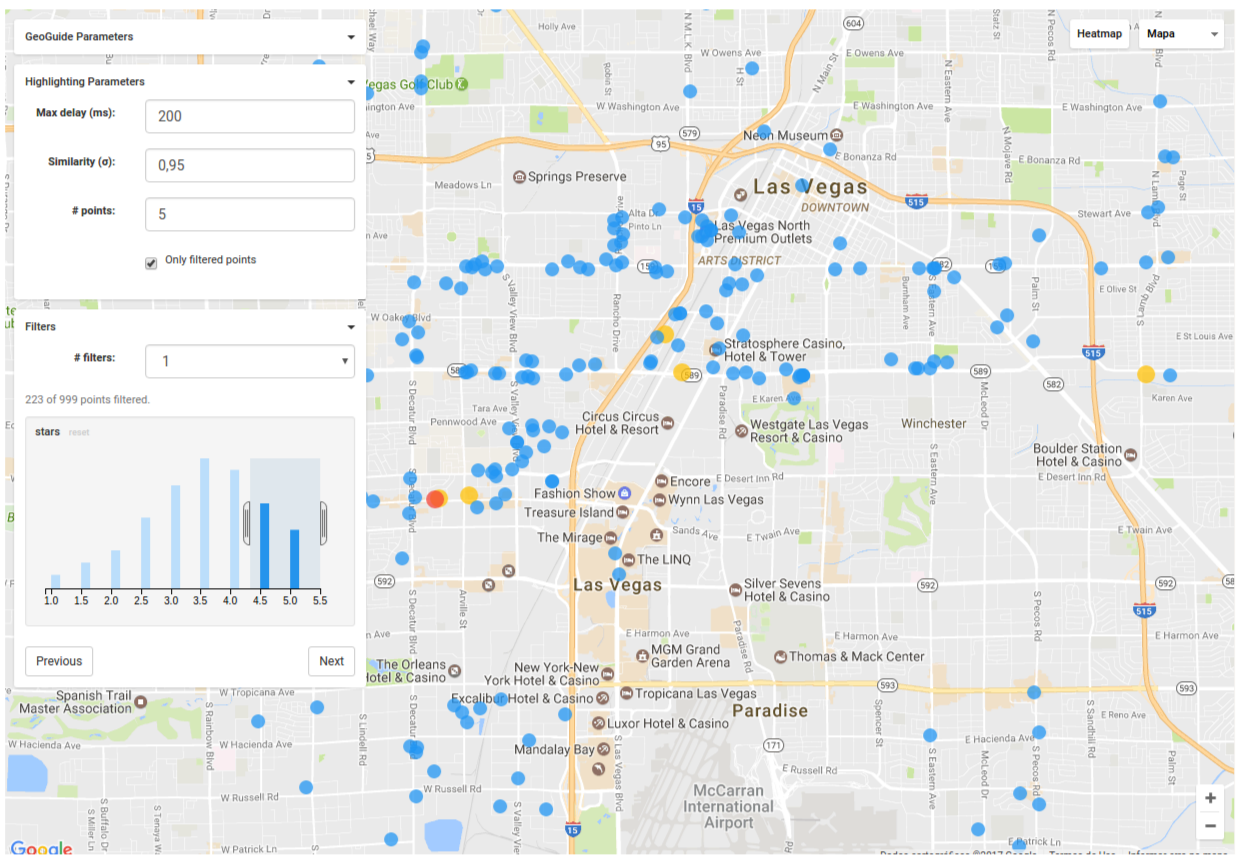
\includegraphics[width=5in]{figs/yelp}
	\caption{\framework\ Image on Yelp Dataset - Las Vegas City}
	\label{fig:yelp}
	\vspace{-10pt}
\end{figure*}


\subsection{Tracking  User's Preferences }

The feedback vector ${\cal F}$ on the schema ${\cal A}$ is initialized by zero. The vector gets updated by ${\cal A}_p$ whenever the analyst shows interest in a geographical point $p$. Feedback vector is always kept normalized, i.e., $\Sigma_{v \in {\cal F}}(v) = 1.0$. Unlike the literature which mainly focuses on explicit feedback (where the analyst should clearly reflect her likes and dislikes), we investigate on implicit feedback. This enables the system to capture {\em what the analyst may miss} instead of what the analyst has clearly investigated before. We consider different ways to capture implicit feedback.

\begin{itemize}[leftmargin=*]
\item {\bf Gaze Tracking.} During spatial data analysis, it is often the case that analysts look at some regions of interest but forget to provide an explicit feedback. For instance in Example~\ref{ex:airbnb}, while Liam is focusing on home-stays close to the Eiffel tower, he also looks at farther locations with easy train access. However, he never clicks on those points. We call this latent signal, {\em gaze}. It shown in \cite{fischer1999investigation} that gaze has a strong correlation with ``user attention''. The signal can be captured by tracking eye movements aka saccades~\cite{arapakis2014user}. We employ {\sc ixLabs} gaze tracking\footnote{\em http://www.xlabsgaze.com/} as it only needs a simple web-cam to capture the gaze signal.
\item {\bf Cursor Tracking.} To address privacy issues of web-cam exploitation for gaze tracking, we consider an alternative option of tracking the mouse cursor. It is shown in \cite{arapakis2014understanding} that mouse gestures have a strong correlation with ``user engagement''. Intuitively, a point receives a positive feedback if the cursor moves around it frequently.
\item {\bf Session Time.} In most spatial datasets, there is a profile page dedicated to each point. Examples are restaurant pages in Yelp and lodging pages in Airbnb. We consider the amount of time that the analyst spends in a page as an implicit feedback. For instance, if the analyst spends few minutes in a page for an Indian cuisine restaurant, this counts as positive feedback for this type of restaurants. 
\end{itemize}


% The point-feedback relevance is neither monotonic nor anti-monotonic. In other words, a highly relevant point to the feedback vector at step $i$ may become totally irrelevant to the updated feedback vector at step $i+1$. The reason is the dynamic nature of the feedback vector which may drastically evolve at each analysis step. For efficiency reasons, we employ a static component of relevance and build indexes to speed up online computations.


% and New York bike-sharing dataset with XXX points.
\section{Application Scenarios}
\label{sec:scenario}

Our application scenarios will describe how \framework\ can be used. First, we present two different scenarios and its datasets. For each scenario, we demonstrate a general view of \framework\ . Then, we describe the sequence of actions to see the highlighted points generated by the environment, and its properties. After, we will present how to align different filter types in order to improve the results. Finally, we will present some results from explicit user's feedbacks, e.g., by choosing different parameters to be highlighted in therms of size and colors.



%\vspace{5pt}
%\noindent{\it Scenario 1.} On New York taxi dataset, we demonstrate how \framework\ can contribute to urban planning and fleet management. We consider an explicit goal of discovering which neighborhoods work the best for which drivers in order to increase the overall availability of cabs in the city. We show how a chain of cab stations can be picked by \framework\ in diverse location of the city.


\vspace{5pt}
\noindent{\it Scenario 1.} On Airbnb dataset, we demonstrate how \framework\ can contribute to approach a lodging of interest based on analyst's feedback. We consider the concrete case of finding a cheap lodging solution with a balcony near Eiffel tower. We will observe how feedback converges the exploration towards the goal very quickly. The analyst, after uploading the possible hosting locations available on Airbnb, she will see some possible places of her interest (in this case, the Eiffel tower) by zooming in on the map. She can filter by price range of her interest, in this case between \textit{\$100} - \textit{\$200} dollars. Then, she can select a host (point in the map) of her interest. Let's consider the place \textit{Chambre luxe 100M Tour Eiffel} (red point in Figure \ref{fig:airbnb} latitude 48.85639, longitude 2.29311), with price of \$ 150 dollars. This place has 1.79 ``reviews per month'' and availability of 362 over 365. She wants to know what other places are similars to this. The analyst sets the environment parameters (\textit{Highlighting Parameters}) with \textit{300 ms} of processing, the minimum similarity of \textit{0.85 $\sigma$} and 10 for the most silimar accommodations from its chosen point.

The result presented in Figure \ref{fig:airbnb} shows the hosts with price in the same range defined in the filter. From this, the analyst can find, between other highlighted point, the place/point ``Paris Eiffel One BR''  with price of \$ 175 dollars per night , 1.19 reviews per month and availability of 295 over 365. This place is a little further from the Eiffel Tower, but still on the same avenue, with similar features and an affordable range based on analyst's first choice.



\vspace{5pt}
\noindent{\it Scenario 2.} On Yelp dataset, e demonstrate how \framework\ can contribute to reach an early consensus on a restaurant. The attendee will observe that his/her preferences will be immediately captured and reflected in future highlights. 

When the analyst decides to explore restaurants similar to Ronald's Donuts in Las Vegas with 4.5 stars, 538 ratings and 1090 check-ins, GeoGuide uses the time the participant observed each restaurant (session time), the selected filters and the profile of the restaurants to be explored in the analysis, which combines implicit and explicit behaviors to suggest new restaurants for observation. After run the environment, GeoGuide highlights the points considered relevant to the participant, that is close to the most analyzed areas and the restaurant that was most observed, with an average evaluation between 4.5 and 5. The points are highlighted in yellow, while the exploded spot is left in red as in Figure  \ref{fig:yelp}. The analyst will then evaluate the options suggested by the GeoGuide to decide whether to choose one of these restaurants or whether to continue exploring.


%\vspace{5pt}
%\noindent{\bf 1. Diversity of parameters in three different datasets. }
%
%\vspace{5pt}
%\noindent{\bf 2. Setting framework variables. }
%
%\vspace{5pt}
%\noindent{\bf 3. Highlighted points generated by the system. }
%
%\vspace{5pt}
%\noindent{\bf 4. Filtering different properties. }
%
%\vspace{5pt}
%\noindent{\bf 5. Implicit and explicit feedbacks. }



\section{Experiments}
\label{sec:experiments}

\vspace{5pt}
To validate our design choices in \framework\ (quality dimensions and feedback capturing), we design a user study with $24$ participants (students in Computer Science). We define a task for each participant and ask him/her to fulfill the task using \framework\ and {\sc Tableau} (as the most advanced off-the-shelf visualization product). Then we measure the number of steps to reach the goal. We define two tasks, {\em T1: finding a point in a requested location} (e.g., find a home-stay in the Central Park area, New York), and {\em T2: finding a point with a requested profile} (e.g., find a cheap home-stay with balcony in Paris.) Participants may begin their navigation from three different starting points: {\em I1: close to the goal}, {\em I2: far from the goal}, and {\em I3: random}. 


\begin{figure}[t]
	\centering
	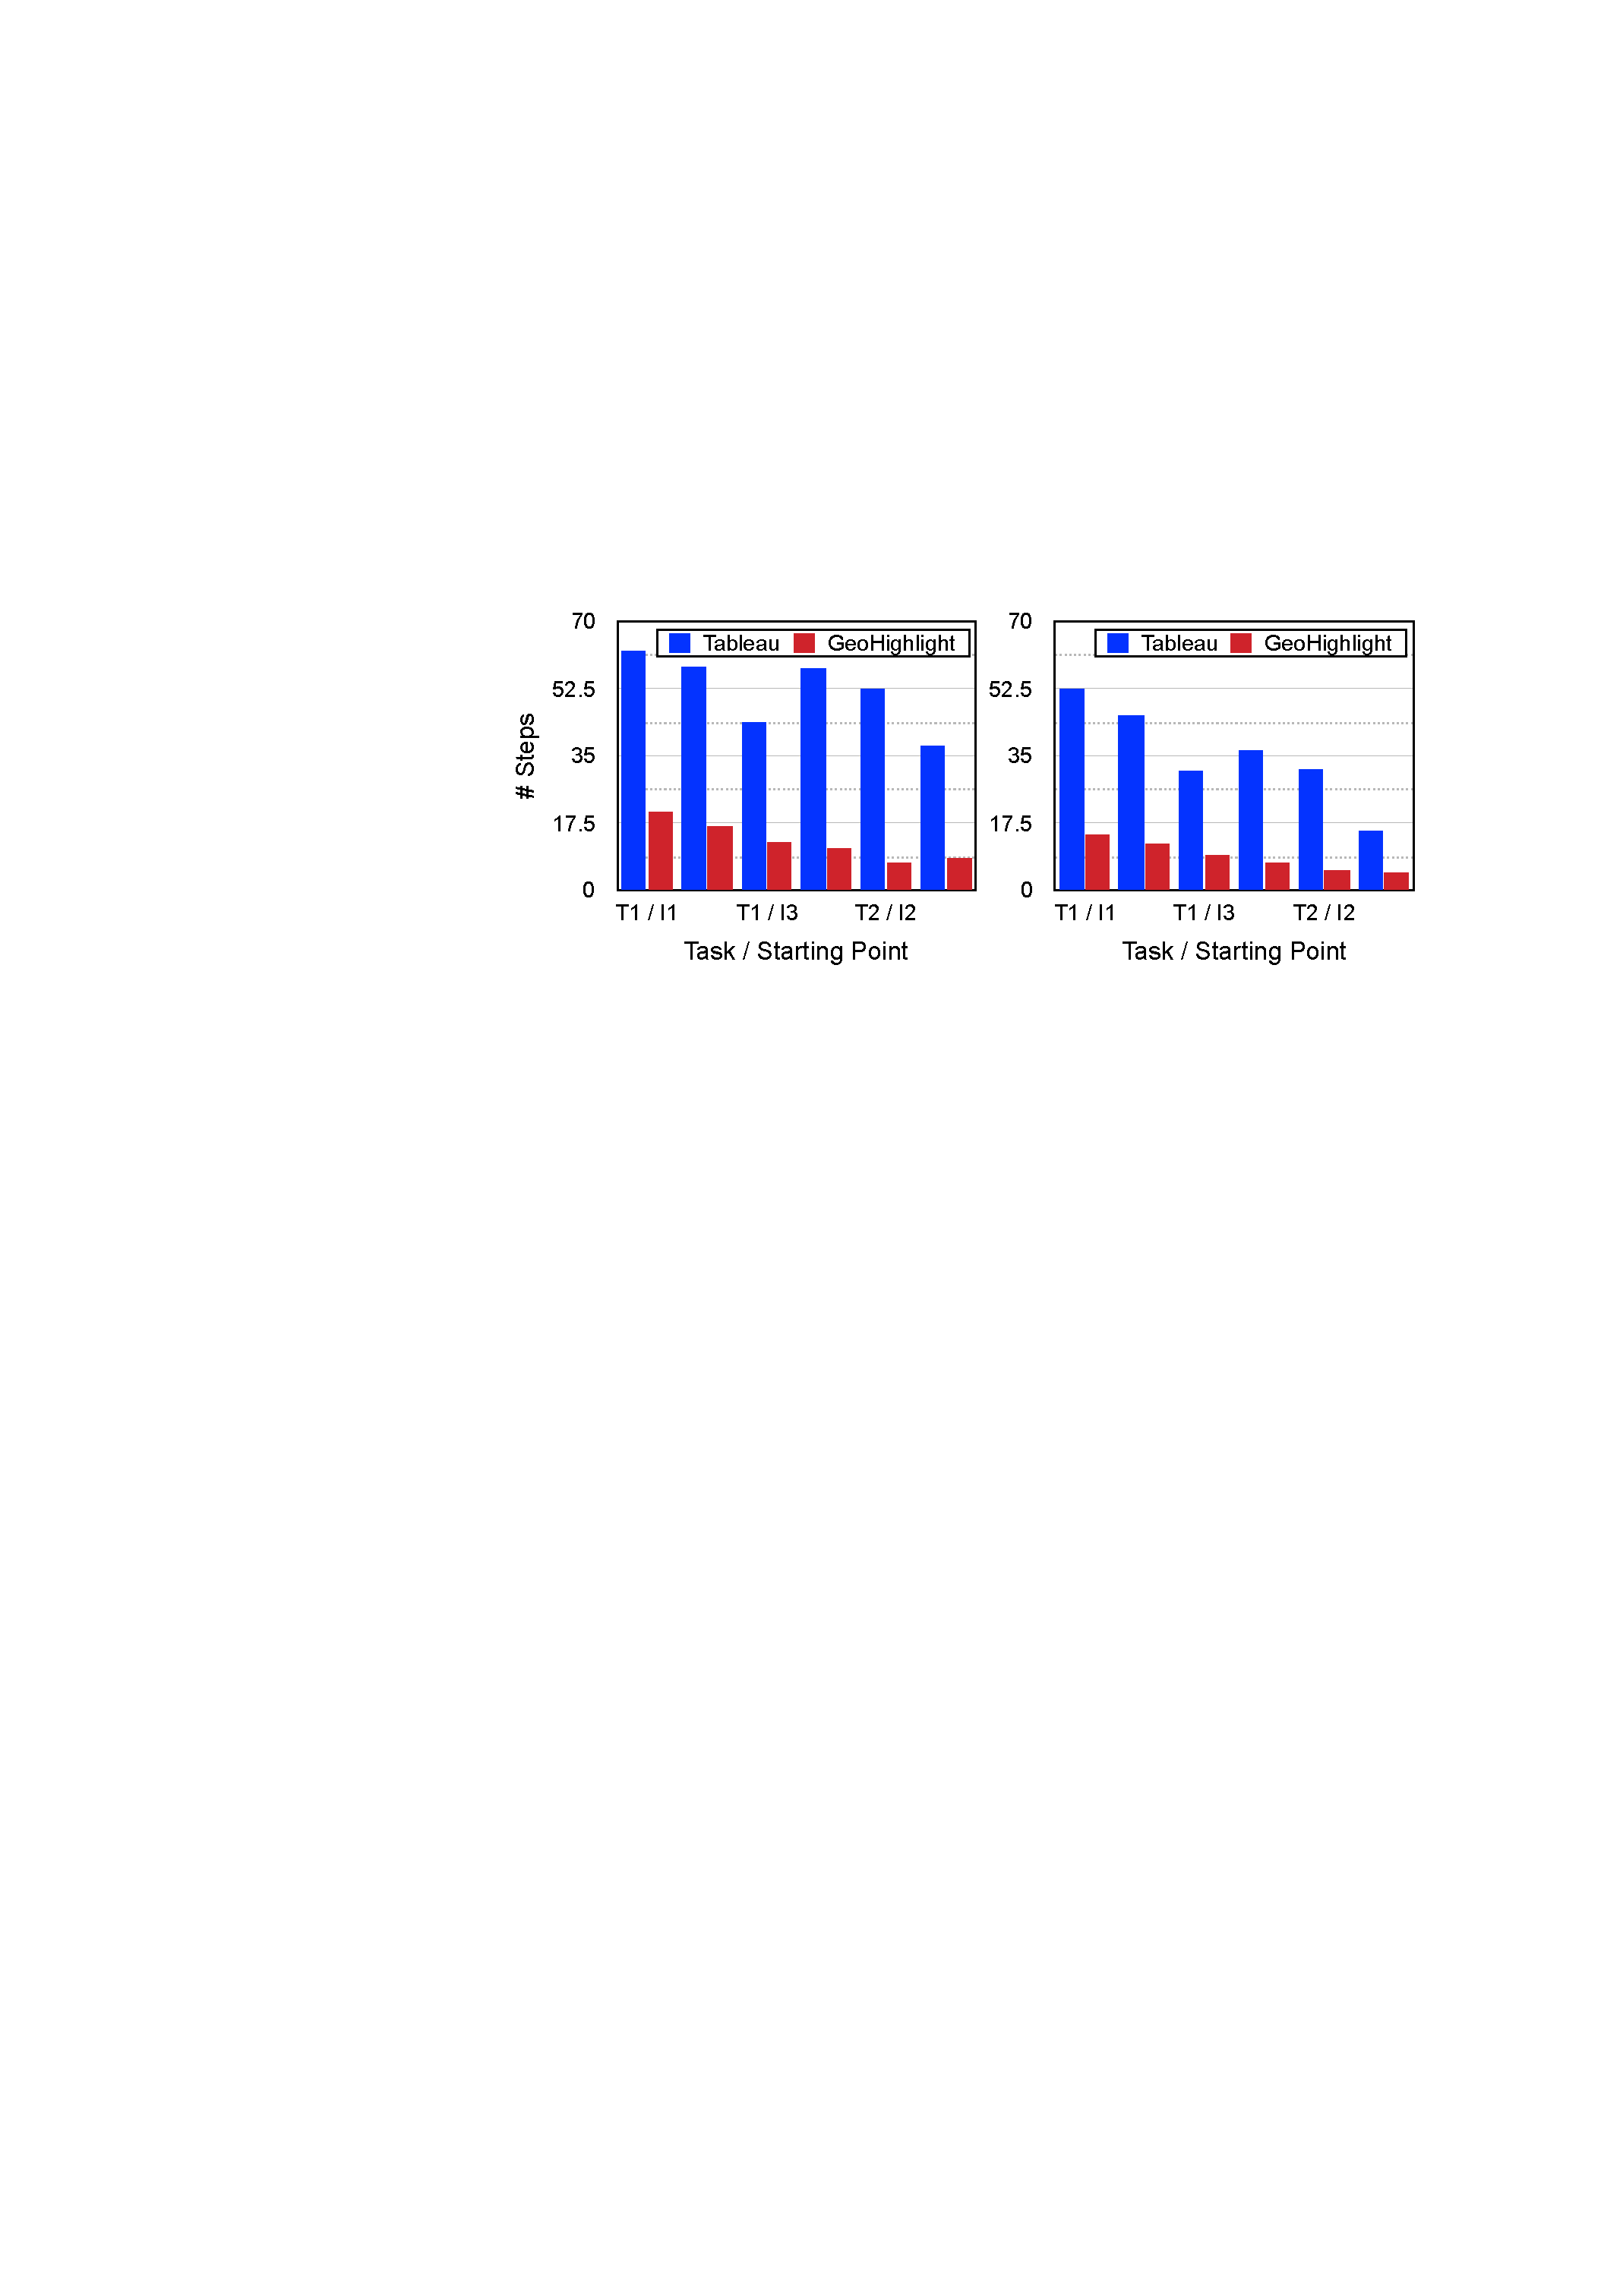
\includegraphics[width=\columnwidth]{figs/userstudy}
	\caption{User Study}
	\vspace{-5pt}
	\label{fig:userstudy}
\end{figure}

In {\sc Tableau}, participants employ filtering and querying tools to reach their goals. In \framework, participants benefit from relevant and diverse highlights and feedback capturing using cursor tracking. Figure \ref{fig:userstudy} illustrates the results of this study. We report results for separate sub-populations: the left figure illustrates the results for novice participants (who don't know the location, be it Paris or New York) and the right figure illustrates expert's results.

We observe that in general, it takes in average 10.7 steps to reach a defined goal in \framework, i.e., 33 steps less than {\sc Tableau}. This shows that the highlighting component equipped with the feedback mechanism helps analysts discover their spatial data and reach to the goal. Level of expertise improves the analysis length in average by 4 steps. Interestingly, starting points do not have a huge influence. It is potentially due to the diversity component which provides distinct options. We also observe that {\em T2} is an easier task than {\em T1}. This is potentially due to similarity component where the analyst can request options similar to what she has already seen and greedily moves to match profiles.




\vspace{5pt}
\framework\ \footnote{\framework\ can be played accessing its environment on http://geoguide.herokuapp.com/.} environment\footnote{A short \framework\ demo can be seen in https://www.youtube.com/watch?v=MTTccStmd0E\&feature=youtu.be} is implemented in Python (as the computation engine), JavaScript D3 (as the visualization engine) and a set of Python libraries. We use and provide some spatial datasets\footnote{https://github.com/placidoneto/Data-Visualization/experiments/inputs} to be run in the framework  : Yelp dataset\footnote{https://www.yelp.com/dataset\_challenge} of restaurant check-ins with 229,907 geographical points, Airbnb dataset\footnote{http://insideairbnb.com/get-the-data.html} for short-term lodging with 4,200,000 points, New York taxi dataset\footnote{https://data.cityofnewyork.us/Transportation/Taxi/mch6-rqy4/data} with 173,179,759 points and citibike New York dataset\footnote{https://s3.amazonaws.com/tripdata/index.html} with different sizes of data. 

\section{Conclusions}
\label{sec:conclusions}

We addressed the problem of guidance and introduced \framework, the first efficient interactive highlighting approach in spatial data. We formulated our problem in form of a constrained optimization and proposed {\sc Highlighter}, a greedy algorithm to highlight $k$-best points for a given point of interest within a time limit. We introduced the discussion of genericness of our approach by materializing few examples from restaurant and apartment rental datasets. We also showed the efficiency and usability of our framework in form of performance experiments and user study. There are several directions of improvement for this work. Specifically, we want to consider an analyst profile vector which is built during interactive steps and will be exploited to return more analyst-tailored results.

Some future extensions include the integration of generic query approach based on \cite{VartakRMPP15}, and we also are going to consider an analyst profile vector which is built during interactive steps and will be exploited to return more analyst-tailored results.


\bibliographystyle{abbrv}
\bibliography{main}


% that's all folks
\end{document}


